\begin{appendices}
\chapter{Chroma Subsampling Artefakte}
\label{appendix:subsampling_artefacts}
\begin{figure}[h!]
    \centering
    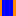
\includegraphics[scale=10]{images/2-1_chroma_artefacts_original.png}
    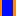
\includegraphics[scale=10]{images/2-1_chroma_artefacts_sampled.png}
    \caption{Artefakte durch Chroma Subsampling}
    \textit{Links: Original, Rechts: Subsampled. Die rechte Kante des blauen Farbblocks liegt in gesubsampleten 2x2 Blöcken, wodurch Artefakte entstehen. Die linke Kante liegt zwischen zwei 2x2 Blöcken, weshalb es zu keiner falschen Darstellung kommt.}
    \label{fig:chroma_artefacts}
\end{figure}

\end{appendices}
